\section{Implementation}

To realize our PGLAS, we have implemented a parallel distributed key/value store, 
PDHT. A novel aspect of this system is its implementation directly on top of the
Portals network interface. The Portals framework provides several low-level 
data abstractions that map nicely onto the PGLAS operations supported by PDHT.

PDHT adopts a one-sided communication model which operates 
with PGAS-like semantics. However, by implementing directly using Portals, we
can take advantage of message-passing features that permit an efficient, 
hardware-offload friendly version of a PGLAS. Some background in the Portals
networking model is helpful in understanding our approach in implementing PDHT.

\subsection{Portals Networking Interface}

% provides several low-level adts for pdht
% one-sided, try to avoid involving processor on the target node
% matching is for MPI, novel application to matching interface
% abstractions for implementing PDHT
% using portals allows us to be hardware offload friendly as compared to 
% traditional PGAS techniques.

The Portals interface provides low-leve data abstractions that can be used to
implement both PGAS and message-passing runtimes. PDHT relies on a one-sided
communication model that aims to avoid processor involvement on the target
node. Portals supports messaging a {\em matching interface} model intended to
support MPI, two-sided matched send/receive pairs. It also provides a
lightweight {\em non-matching} interface that is intended to support one-sided
communications without the need for the matching and ordering semantics
required by MPI. Our implementation uses a novel application of the Portals
matching interface to provide a one-sided model that is the basis of the PDHT
PGLAS. It is useful to describe several Portals concepts and abstractions to
understand the implementation approach used by PDHT.

% use figure* to span both cols
\begin{figure}[ht]
  \centering
  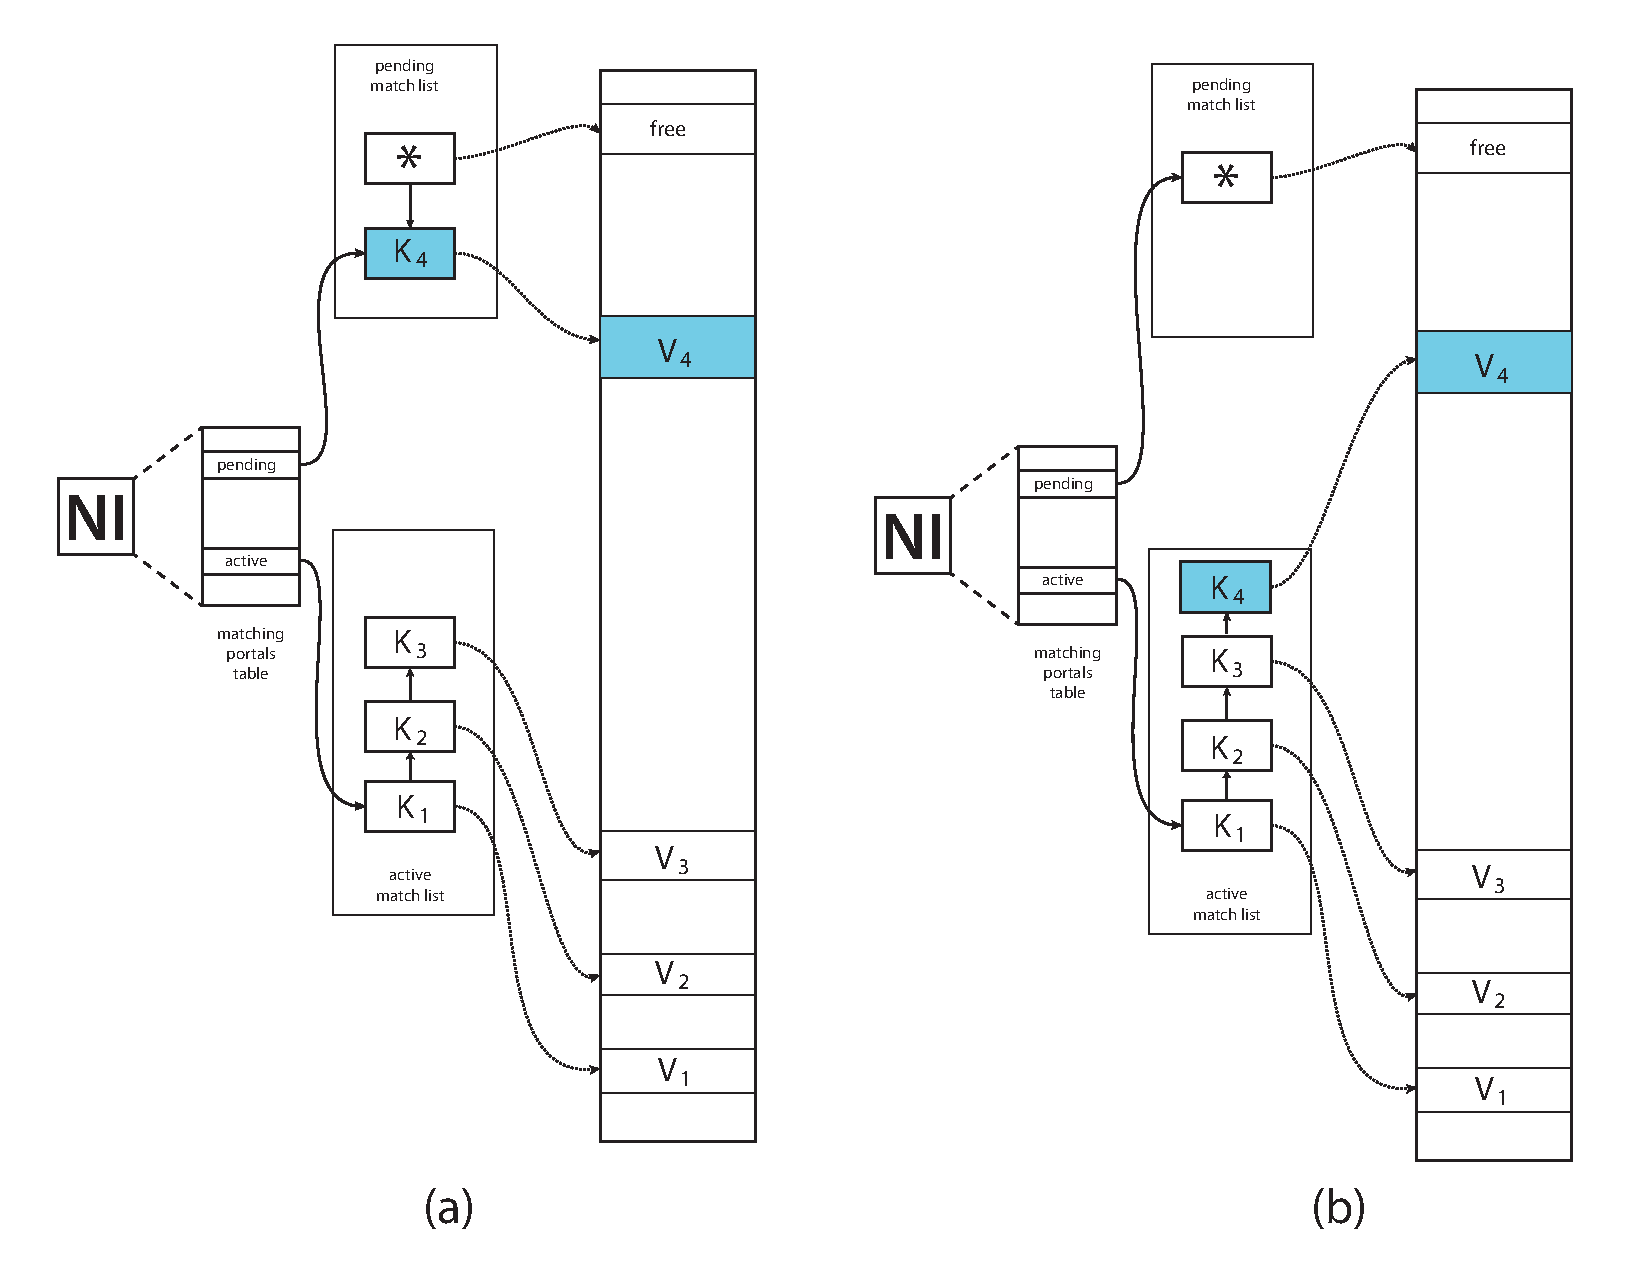
\includegraphics[width=3in]{figs/put_smaller}
  \caption{Portals data abstractions used in for a matching interface {\tt put} operation}
  \label{fig:put}
\end{figure}

Portals defines two distinct roles for communication oerations. The {\em
  initiator} role is assumed by the process that issues a Portals put, get, or
atomic operation. The {\em target} role is assumed by the process that receives
these operation requests and is responsible for performing the operation or
sending the requested data.

The Portals {\em network interface} (NI) data structure is a per-process
abstraction of a physical network interface and is configured as a
matching or non-matching interface. The NI is associated with both
initiator and target roles. Initiator processes define a {\em memory
  descriptor} (MD) -- a region of memory used for the put/get/atomic
operations as well as ancillary structures used to track communication
events (such as completion) for these operations.

Target processing is expressed in terms of a {\em portal table}. There is one
portal table for each NI, containing multiple entries that separate and
classify communication channels between endpoints.  Each {\em portal table
  entry} (PTE) is identified by a unique index into the Portal table. The index
for a specific PTE is required for all Portals communication operations. Each
PTE maintains a list of memory regions that are valid for communication
operations as well as an event queue which is used to track target-side
asynchronous notifications.  Some completion information and notifications may
only be visible to the initiator and not the target, or vice versa.

A PTE using the matching interface maintains a list of match-list entries (ME).
Each ME specifies a set of matching criteria and a memory region associated
with the entry. If the match criteria are satisfied, the communication
operation commences working on corresponding memory region. Matching criteria
consist of multiple parameters, including a a 64-bit {\em match bits} field
that must be an exact match in order for an incoming request to to proceed
with the given ME. For example, a process may post an {\tt MPI\_Recv()} which
creates a new ME on the target PTE with a specific match bits value. Later,
another process would issue an {\tt MPI\_Send()} communication request with
the same match bits that corresponds to the previous receive.

Portals also specifies {\em event queues} and {\em event counters}
used to track data movement in and out of memory regions used by Portals
operations. Events and counters can also log failure events and
other information. Counting events are lightweight operations and only
record the success or failure of a given operation. Full events incur
more overhead but contain detailed information about the event and
the corresponding communcation operation.

Event queues may be associated with an MD (initiator-side) or a PTE
(target-side). Event counters are also able to track both initiator
and target events. In contrast to target-side event queues, an event
counter may be associated with a single entry in the matchlist (an ME), 
rather that for an entire PTE. PDHT typically uses lightweight counting
events to track successful completions and full events to track specific
failures. Detailed descriptions of how event queues and counters are used
within PDHT is discussed below.

Figure~\ref{fig:put} shows a visual representation of the target-side
structures used in an example {\tt PtlPut()} operation using the matching
interface. We assume that the initiator has issued a {\tt PtlPut()} operation
with some data, a PTE index and the match bits set to 74. Upon receiving the
request, the target process searches the match list for the given PTE until a
74 is found or the end of the list is reached. Once a match has been found the
payload data of the {\tt PtlPut} is copied into the memory region associated
with the ME. The completion of this operation may cause an event to be appended
to the PTE event queue or the ME success counter to be incremented. 
Lastly, an acknowledgement message is sent back to the initiator, posssibly
generating another full or counting event associated with the MD that
was used to initiate the {\tt PtlPut} operation.

Portals supports two lists for messages, the unexpected list and priority list. 
These are used for the unexpected message queue and posted recieve queue in MPI. Portals supports the 
searching of the local unexpected list through PtlMESearch because of the need to match a MPI\_Recv
call with a message on the local unexpected message queue. However, Portals does not support the searching of 
the local priority list through PtlMESearch. We added functionality to PtlMESearch so it looks for matches
on the local priority list instead of the unexpected list, if specified. This allowed us to find hash table entries without 
calling PtlGet when hash table entries were stored locally. This lead to a 10x speed up in local hash table 
lookups.


\subsection{PDHT Implementation}

% serial vs. parallel approaches
Hash tables can be implemented with a myriad of different techniques, but are
traditionally implemented sequentially as an array of pointers to objects.
Parallel implementations typically distribute table data across nodes,
requiring that the hash table stores the entire object and not simply a
reference. 


A primary motivation for using a one-sided approach is to allow
RDMA-based memory accesses to fetch remote data without interupting
the processor core on the far end. We can take advantage of NIC
hardware offload to a greater extent than conventional PGAS approaches
by using low-level communication primitives provided by the Portals 4
network interface specification. Portals defines a number of
abstractions and concepts that are necessary to understanding the PDHT
implementation.


\subsection{PDHT Programming Model}


% parallel programming model
%  - key/value pairs
%  - object can be located anywhere distributed memory, governed
%     solely by hash function
%  - hash function maps key -> rank/offset tuple
%  - two primary operations put/get
%     - if put yields a collision, then object is placed in next
%        available bucket
%     - get returns object, probing as necessary
 
The PDHT system provides a distributed key/value store within a
high-performance computing cluster. A hash function maps the object
key to a rank and offset tuple, identifying each distinct location
within the hash table. PDHT provides the two primary {\em put} and
{\em get} operations to store and fetch items from the table. Since
multiple keys may hash to the same table location (a collision), PDHT
implements a linear probing behavior. If a {\em put} yields a
collision, the object is then placed in the next available bucket on
the same processor rank. The {\em get} operation also checks for
collisions and searches accordingly. 

% considerations:
%  - two-sided communication not amenable to hash table implementation
%  - one-sided will rely on MPI-2+, UPC, or some other PGAS-ish
%     approach
Two-sided communication is not inherently amenable to implementing a
high-performance hash table. Hash tables rely on fine-grained, random
data access which makes a message-passing based implementation
challenging. Several existing approaches have been built upon
one-sided models using MPI-2, UPC, and other PGAS approaches.

\begin{figure}[ht]
  \centering
  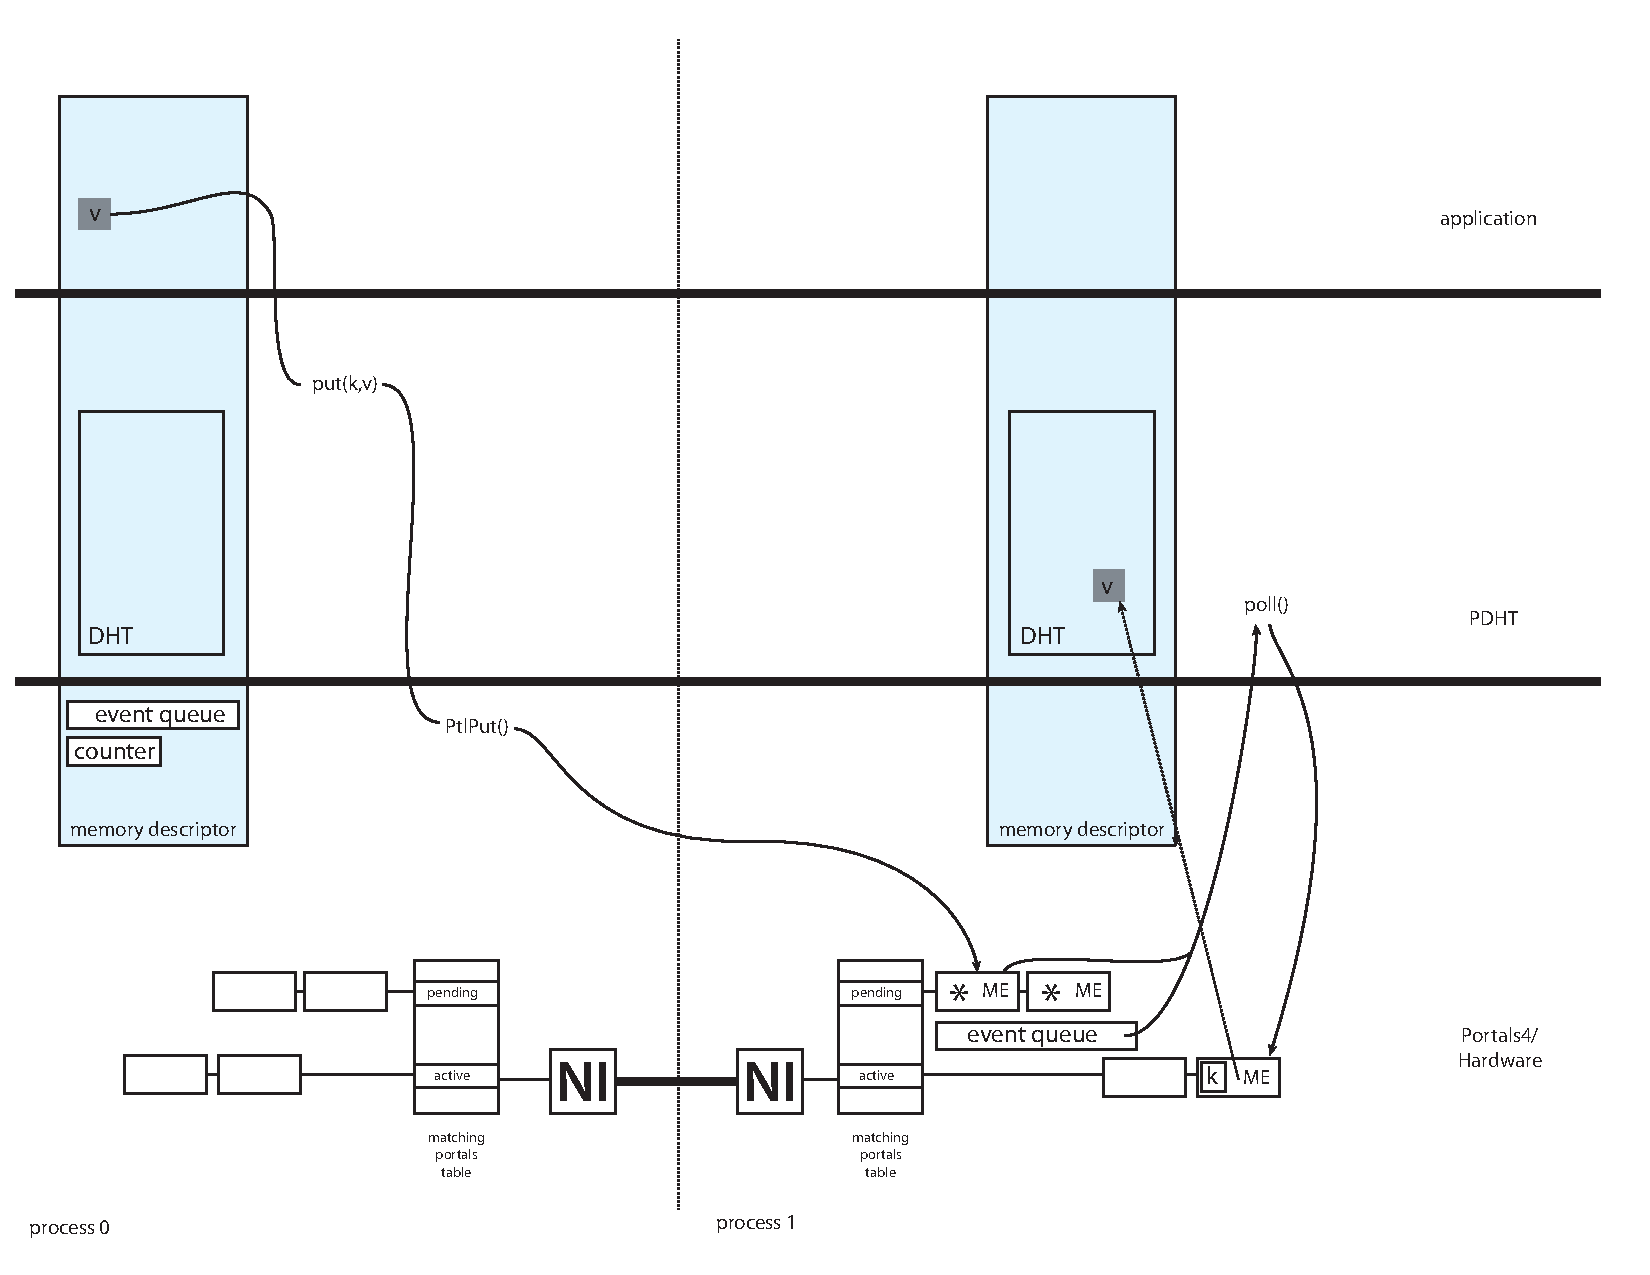
\includegraphics[width=3in]{figs/hwsw}
  \caption{Hardware/Software Abstractions}
  \label{fig:hwsw}
\end{figure}

% implementation
%  - array of objects + metadata
%  - pending ME list 
PDHT supports multiple hash tables per-process. Each hash table is
treated as a distributed array of value objects and a small amount of
metadata per entry. Upon initialization, PDHT opens a Portals NI with
two distinct portal table entries, one for {\em pending} match list
entries and another for {\em active} match list entries. The pending
match list is filled with a number of entries that will match any
incoming communication request. Each match list entry corresponds to a
local memory region that can contain a single entry in the hash table
array structure.

The key idea within PDHT is to create a match list entry (ME) for each
active element in the hash table. The hash function maps the key to a
64-bit value used as the match bits field for the Portals
communication request. By relying on the matching interface to handle
hash entries, much of the servicing of a get request can be relegated
to Portals, which in turn rely on hardware acceleration.

% put operation
%  - run hash to determine rank/offset
%  - figure 1
%  - active ME list
%  - migration from pending to active

To insert a new element into the hash table, the process first hashes
the key, giving both the target processor rank and the 64-bit match
bits field used for the value. Next, the process performs a one-sided
put operation on the pending PTE, using one of the wildcard entries on
the match list. The hash table value data is communicated and stored
into the memory region defined by the match list entry. As can be seen
in Figure \ref{fig:put}a, the table entry data resides on the owner
process, but the match-list entry is still resident on the pending
PTE, rather than the active one. To complete the put operation, the
used up entry on the pending PTE needs to be replaced with a new empty,
wildcard ME and the new hash table object needs to have an entry on
the active PTE, with the match bits set to correspond to the hashed
key. This state can be seen in Figure \ref{fig:put}b. 

% - polling approach
The most straightforward approach to moving the ME from the pending 
match list to the active list is by relying on a progress
thread. Portals provides blocking wait and polling routines to check
for new event notifications or counter changes. When a process
receives a put operation and updates the pending match list, a Portals
event is generated and appended to the event queue. When the progress
thread sees this event, it creates a replacement wildcard entry for
the pending queue that references an empty element in the hash table
array. It also creates a new ME with the appropriate match bits and
appends it to the active list. Any subsequent get requests will be
able to find a match in the active PTE.


% - triggered append approach


% get operation
%  - run hash
%  - issue PtlGet from active list
%  - check for collision



%  - custom hash functions 
%  - 64-bit hash space, rather than array bucket
%      - detach key -> array size dependency
%      - lower collision rates

% other operations
%  - iteration
%  - non-blocking / bundled puts/gets
%  - interoperability


%%% Local Variables: 
%%% mode: latex
%%% TeX-master: "paper"
%%% End: 
